\section{Mes développements notables sur \textsc{Sigma}}

Dans cette partie, je vais évoquer certains développements intéressants sur lesquels j'ai travaillé durant mon apprentissage au sein de \textsc{Disa}.

\subsection{Configurateur de devis}

\subsubsection{Le besoin exprimé par les deviseurs}

Nous avons développé, au sein de \textsc{Sigma}, un module permettant aux deviseurs de créer des devis.
Le développement de ce module fut long et complexe, il était déjà en cours lors de mon arrivée à \textsc{Disa} et se poursuivit encore sur plusieurs mois.
À terme, l'outil de génération des devis créé était fonctionnel et permettait bien de créer des devis.
Cependant, après une présentation de cet outil aux deviseurs, ceux-ci nous ont demandé s'il était possible de leur offrir un outil permettant de créer une version simplifiée d'un devis, contenant seulement les informations minimales.
Le but de cet outil serait de permettre la création de devis de manière simplifiée et plus rapide.

Les devis créés par les deviseurs sont souvent très semblables et c'est donc une perte de temps pour eux d'avoir à saisir les mêmes informations pour plusieurs devis différents.
Le but était donc de garder le module initial pour la création de devis complexes et d'utiliser un nouvel outil pour la génération de devis simples, composés d'opérations similaires.

Afin de concrétiser leurs idées, nous avons demandé aux deviseurs de créer un fichier \textsc{Excel} représentant leur vision de ce configurateur.
Avec M. \textsc{Palier}, nous avons relevé de nombreux points qui manquaient de clarté, un certain nombre d'incohérences et surtout des fonctionnalités indispensables qui avaient été omises dans ce document.
Nous nous sommes donc entretenus de nombreuses fois avec les deviseurs afin de corriger et améliorer cette ébauche.
Nous sommes finalement arrivés à une version qui nous semblait réalisable sous \textsc{Sigma}.

\subsubsection{La solution apportée}

J'ai effectué la conception et le développement de ce configurateur lors de ma seconde mission en entreprise.
L'objectif du configurateur de devis était de simplifier le travail des deviseurs.
J'ai donc fait en sorte que celui-ci ne comporte qu'une seule fenêtre et se présente de la manière la plus claire possible.

Le configurateur ne devait gérer que les cas de devis composés uniquement d'impositions constituées d'une pose unitaire.
Une imposition constituée d'une pose unitaire est le cas le plus simple existant.
La pose unitaire signifie que sur chaque feuille imprimée il n'y a qu'un seul motif, celui-ci est répété sur toutes les feuilles.
Les autres cas sont les multiposes et les amalgames : les multiposes consistent en l'impression d'un même motif en plusieurs exemplaires sur chaque feuille et les amalgames consistent en l'impression de plusieurs motifs différents sur chaque feuille.

Le configurateur est constitué de quatre tableaux.
\\
\begin{enumerate}
    \item Le premier tableau permet de gérer les impositions.
    On peut en ajouter ou supprimer, on peut sélectionner le type d'impression, la matière d'impression, le format et plusieurs autres informations.
    La saisie des informations au sein de ce premier tableau entraîne l'ajout automatique de plusieurs opérations lors de la validation du configurateur.
    La saisie entraîne aussi l'ajout automatique de lignes prérenseignées dans le second tableau.
    
    \item Le second tableau permet de gérer la nomenclature du devis.
    La nomenclature du devis permet de renseigner la liste des outils, matières, encres et accessoires qui seront utilisés lors des étapes de production.
    La majorité des lignes de ce tableau sont ajoutées automatiquement lors de la saisie des informations du premier tableau.
    L'utilisateur peut tout de même ajouter manuellement des lignes au sein de la nomenclature s'il le souhaite.
    
    \item Le troisième tableau permet de gérer les phases de sous-traitance.
    Toutes les lignes de cette table doivent être générées manuellement, elles permettent d'indiquer si certaines opérations du devis doivent être sous-traitées.
    Il faut donc renseigner le temps et le prix de chaque sous-traitance.
    
    \item Le quatrième tableau permet de gérer les opérations manuelles.
    Ce sont des opérations dites de <<~kittage~>>, elles sont réalisées après les phases d'impression et permettent le conditionnement du produit en préparation de sa livraison au client.
    Ici, l'utilisateur ne peut pas ajouter ou supprimer de lignes, mais seulement renseigner une estimation des temps que chacune de ces opérations prendra.
\end{enumerate}
~\\

Sur l'image ci-dessous on peut voir la fenêtre du configurateur telle qu'elle l'était à ce moment du développement.

\FloatBarrier
\begin{figure}[h!]
    \begin{center}
        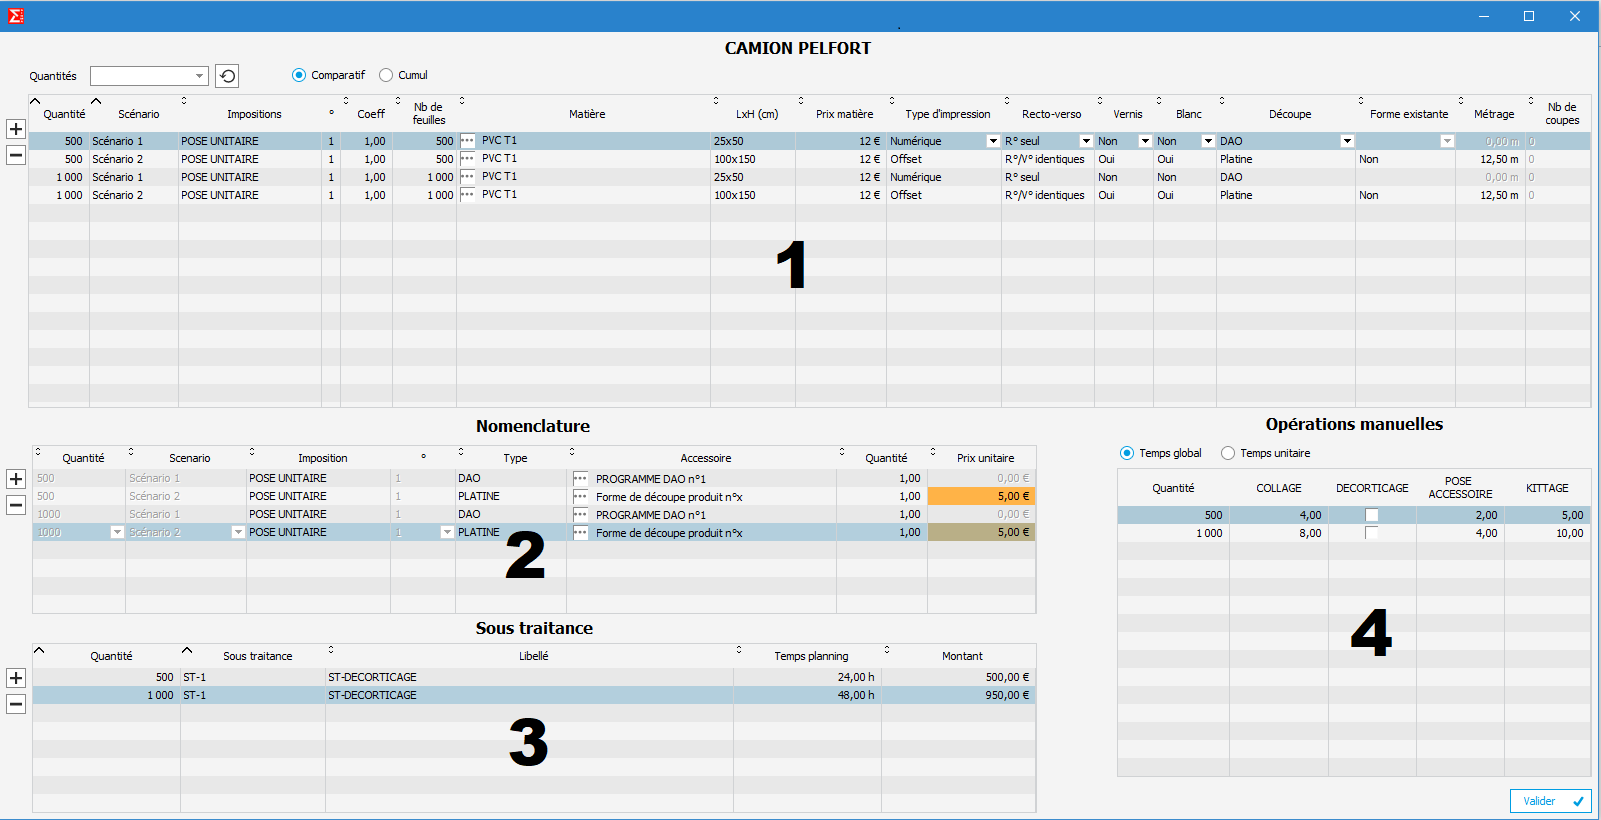
\includegraphics[width = 0.9\textwidth]{conf}
    \end{center}
    \caption{Configurateur de devis avec les tableaux numérotés}
    \label{figure:conf}
\end{figure}
\FloatBarrier

La partie la plus complexe et laborieuse du développement fut pour gérer l'étape de validation du configurateur.
En effet, la fenêtre est simple, comporte peu d'informations et permet de simplifier grandement le travail des deviseurs, en revanche cela complexifie beaucoup le traitement d'enregistrement des informations en base de données.
Afin de générer un devis à partir des informations présentes dans les quatre tableaux, il faut renseigner une quinzaine de tables en base de données, en prenant garde à bien relier tous les éléments entre eux.

Pour un tel travail de développement, il est primordial de s'organiser afin de ne pas perdre le fil.
Sans organisation il n'est pas rare de se lancer dans un long développement de plusieurs heures, voire jours et, à terme, de ne plus comprendre comment son code fonctionne et de devoir tout recommencer plus méthodiquement.

Afin d'aborder ce développement, j'ai donc schématisé toutes les relations de la base de données sur un cahier, en préparant ainsi par la même occasion l'ordre de chaque import en base de données.
Car en plus de devoir relier tous les enregistrements entre eux, il faut aussi faire attention à les ajouter dans le bon ordre afin de garantir une cohérence des données.
Une fois ce travail effectué, j'ai pu développer le traitement de validation, j'ai également commenté proprement le code afin de permettre une reprise et modification simple du code à l'avenir.

Je suis parvenu à terminer le développement du configurateur avant la fin de ma seconde mission.
L'outil était fonctionnel et répondait au besoin des deviseurs tel qu'il fut décrit initialement.

\subsubsection{Les raisons de l'échec et abandon de ce projet}

Lors de mon retour pour la troisième mission en entreprise, on m'annonça que le configurateur de devis était peu utilisé, car de nombreux cas très courants n'étaient pas gérés.
Ces cas étaient jugés complexes et c'est pourquoi ils n'avaient pas été pris en compte pour le configurateur, puisque l'objectif n'était de l'utiliser que pour les cas courants et simples.

Les deviseurs avaient donc surestimé le taux de réalisation de devis simples et nous n'étions pas parvenus à détecter ce problème plus tôt, avec M. \textsc{Palier}.
Nous étions tout d'abord opposés à l'idée de modifier le configurateur pour prendre en compte ces cas complexes, mais nous sommes parvenu au constat que la grande majorité des devis ne sont finalement pas composés de cas simples, au contraire.
Par conséquent, bien que fonctionnel, l'outil n'était pas assez adapté aux besoins des deviseurs et n'était donc pas utilisé.

Nous avons donc décidé de prendre en compte plus de cas de figure.
Parmi les cas de figure supplémentaires qu'il fallait gérer se trouvait la gestion des multiposes ainsi que des amalgames.
La gestion de tous les nouveaux cas de figure complexifia énormément le traitement de génération des lignes de nomenclatures automatique.
Cela complexifia par la même occasion le traitement des enregistrements en base de données.

Le principal souci causé par l'ajout de tous ces cas de figure est que nous avions spécifiquement décidé de ne pas les gérer.
La totalité de la conception et du développement de l'outil a donc volontairement été effectuée sans les prendre en compte.
La modification du configurateur s'est donc effectuée dans de mauvaises conditions, il était impossible d'ajouter les fonctionnalités demandées sans entraîner de grosses modifications au traitement de base.

Malgré les tentatives, il fut impossible d'ajouter les fonctionnalités sans provoquer des bugs empêchant totalement l'utilisation du configurateur.
Il a alors fallu refuser de faire ces modifications.

Le configurateur ne répondant toujours pas aux besoins des deviseurs, nous avons préféré mettre le projet de côté afin de ne pas perdre plus de temps.

\subsubsection{Les solutions compensatoires développées}

Même si le configurateur de devis ne fut pas un succès, nous avons tout de même développé plusieurs fonctionnalités permettant de simplifier le travail des deviseurs.

Parmi ces fonctionnalités, ils ont la possibilité de créer des devis à partir d'une copie de la gamme\footnote{La gamme d'un devis est la liste de toutes les opérations de fabrication à effectuer.} ou de la nomenclature d'un autre devis.
Ainsi, cela leur permet de créer très rapidement tous les devis similaires.
Nous avons aussi généré des gammes et nomenclatures type qui correspondent à la majorité des cas de devis.
Celles-ci servent de modèle au devis et nécessitent peu de modifications de la part des deviseurs afin de les adapter aux besoins du client.

Bien que le configurateur fut un échec et que nous avons ajouté des fonctionnalités permettant de soulager le travail des deviseurs, l'idée de la création d'un nouveau configurateur est toujours présente.

\subsubsection{Leçons tirées de cette expérience}

L'échec du développement du configurateur de devis est principalement dû à la compréhension seulement partielle du besoin des utilisateurs et à une étape de récolte du besoin qui fut complexe.
Le développement aurait pu être rendu plus simple si nous nous étions rendu compte plus tôt que la gestion des cas jugés simples n'allait pas suffire à satisfaire les besoins des deviseurs.

Étonnamment, cet échec est le seul que j'ai rencontré lors de mon apprentissage au sein de \textsc{Disa}, alors que c'est un module pour lequel nous portions justement une attention toute particulière à la compréhension du besoin.
Nous savions, avec M. \textsc{Palier}, que la réalisation d'un tel configurateur était ambitieuse et allait être laborieuse et nous voulions alors nous assurer de bien concevoir l'outil, afin de ne pas nous retrouver dans une mauvaise situation par la suite.
C'est pourtant exactement ce qui est arrivé.

Cela montre que même lorsque l'on pense avoir assez clarifié les besoins des utilisateurs, il est nécessaire de prendre ses précautions et de s'entretenir avec eux régulièrement, afin de leur faire valider l'avancement du développement et de pouvoir déceler les éventuelles divergences entre le produit développé et le besoin réel.

\newpage
\subsection{Planning de production}

\subsubsection{Le besoin d'informatiser le processus de planification}

Afin de planifier la production de l'entreprise, les responsables de la production utilisaient depuis de nombreuses années de grands tableaux permettant d'accueillir des papiers sur lesquels étaient indiquées les informations des phases de fabrication.
Ces tableaux permettaient une organisation de toutes les phases, par machine et par jour, ainsi, lorsqu'un ouvrier voulait savoir ce qu'il avait à faire, il devait venir voir les phases sur le tableau et ensuite récupérer le dossier papier correspondant à l'OF\footnote{Ordre de fabrication, document présentant la liste des phases de fabrication} en question, puis retourner à sa machine.

\FloatBarrier
\begin{figure}[h!]
    \begin{minipage}[c]{0.6\textwidth}
        \begin{center}
            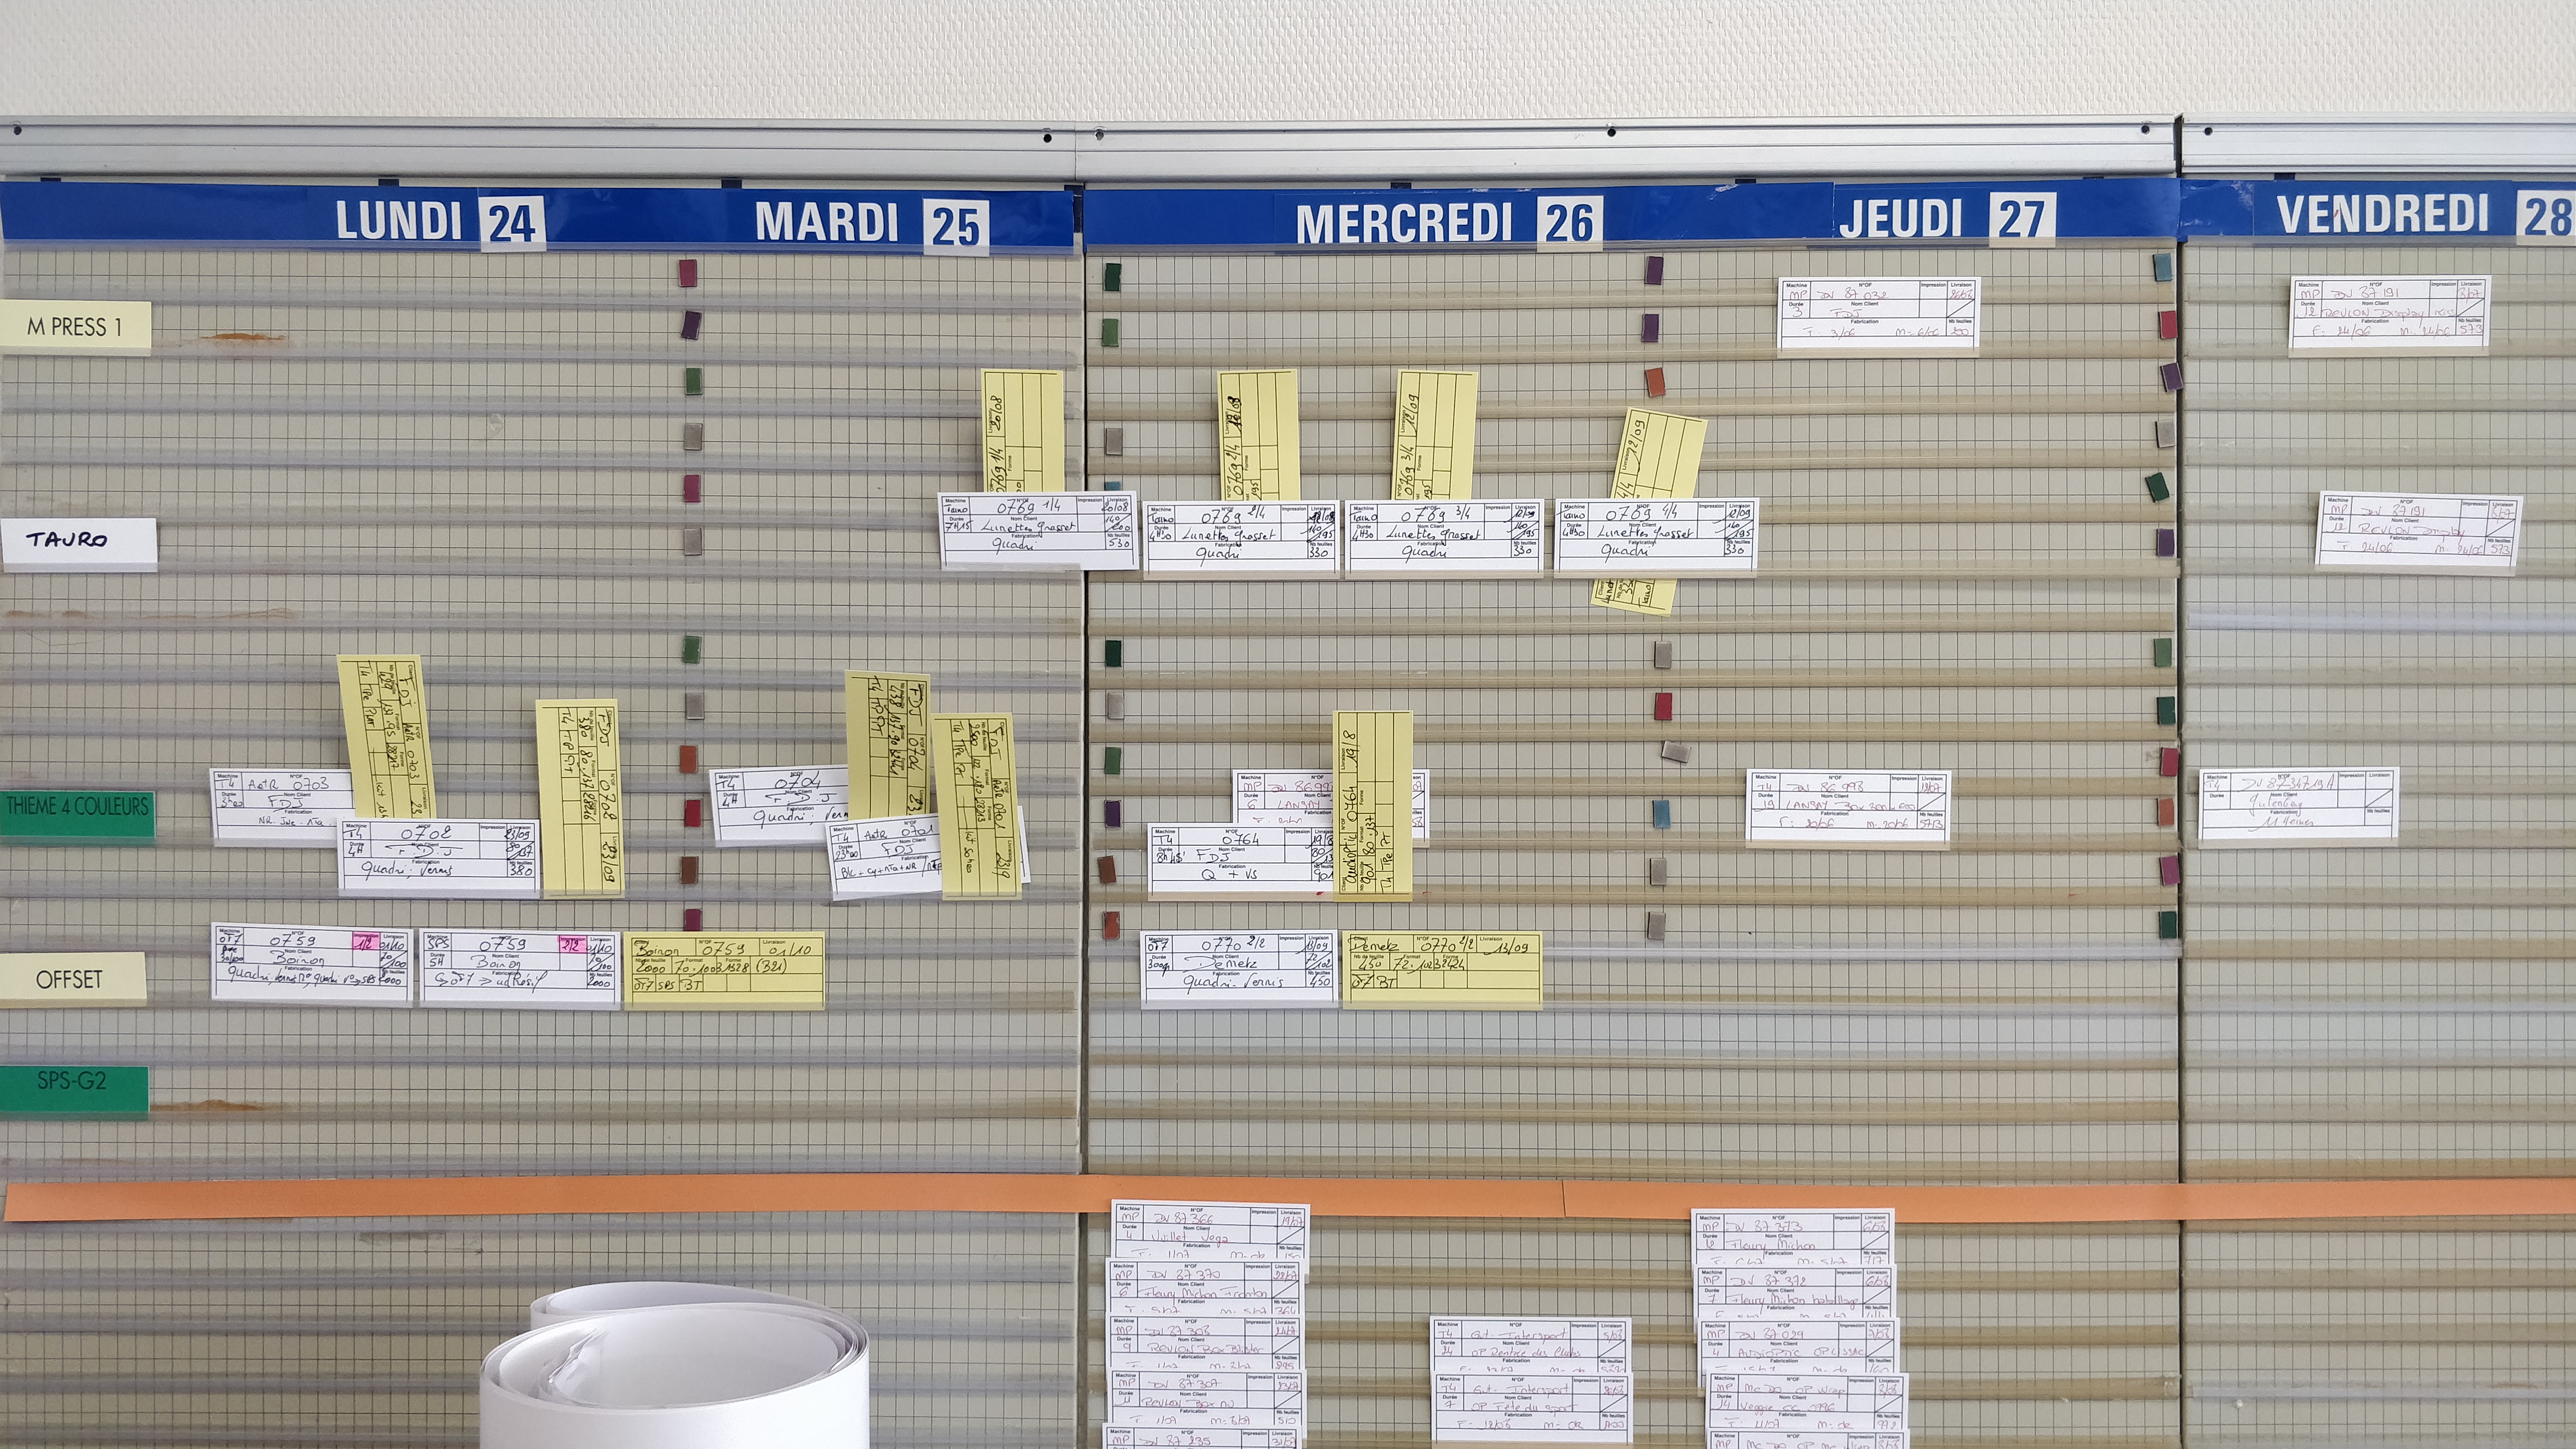
\includegraphics[width = 0.9\textwidth]{planning}
        \end{center}
    \end{minipage}\hfill
    \begin{minipage}[c]{0.4\textwidth}
        \caption{Exemple d'une petite partie d'un tableau de production}
        \label{figure:planning}
    \end{minipage}
\end{figure}
\FloatBarrier

Avec le projet \textsc{Sigma}, M. Palier entendait supprimer au maximum les besoins d'impression des documents de fabrication.
Chaque dossier de fabrication pouvait rapidement atteindre entre 10 et 20 pages, le nombre de dossiers pouvant aller jusqu'à plusieurs dizaines par jours, la quantité de papier et d'encre utilisée était énorme.

Il fallait donc remédier à cette consommation excessive de papier et d'encre.
Cela passe par le développement de deux outils~:~le premier est l'outil de planning de production et le second est le développement de la SFAO sous \textsc{Sigma}, décrit dans la prochaine section.

\subsubsection{Le développement du planning}

J'ai effectué le développement du planning lors de ma quatrième mission en entreprise, le but de ce planning était de remplacer les tableaux physiques.
Nous avons décidé de développer un planning sur lequel les responsables de la production pourraient organiser toutes les phases de fabrication.
En parallèle, il fallait développer la SFAO en s'assurant que les deux outils puissent fonctionner ensemble et en même temps.
L'organisation des phases de production doit, par exemple, entraîner en direct l'affichage des phases à réaliser pour chaque machine sur la SFAO.
Remplacer le tableau physique a permis de simplifier le travail des ouvriers qui n'ont plus à traverser toute l'usine pour prendre connaissance des prochaines tâches à effectuer.

Nous avons décidé de présenter le planning de fabrication de manière assez similaire au tableau physique, c'est-à-dire les machines sur la gauche et les jours de la semaine en haut.
Les utilisateurs peuvent glisser les phases depuis un tableau sur la droite directement à l'endroit souhaité dans le planning.
L'ordonnancement des phases se fait manuellement sur le planning.

\FloatBarrier
\begin{figure}[h!]
    \begin{center}
        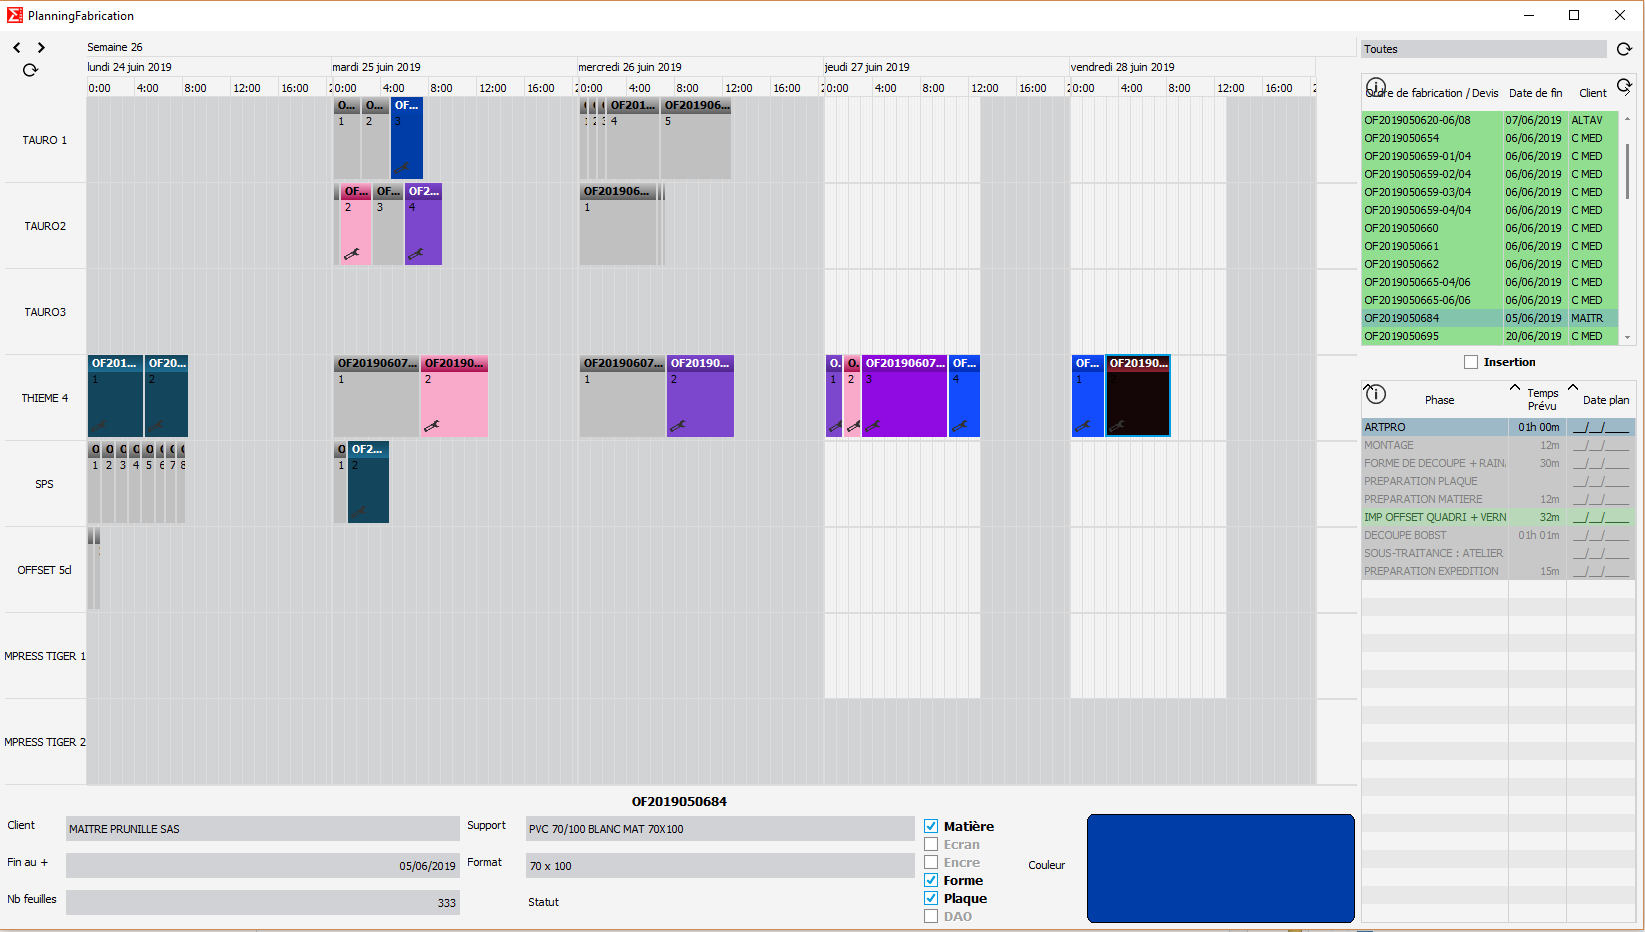
\includegraphics[width = 0.9\textwidth]{planning_1}
    \end{center}
    \caption{Aperçu du planning de fabrication intégré à \textsc{Sigma}}
    \label{figure:planning_1}
\end{figure}
\FloatBarrier

Bien que le planning soit très simple d'utilisation, ce qui fut long dans le développement de celui-ci fut la création de tous les traitements permettant une organisation fluide des phases au sein du planning.
Car, lorsque l'on souhaite déplacer une phase il faut, en arrière-plan, gérer la réorganisation de toutes les autres phases sur cette machine.
Il faut aussi prendre en compte les heures d'utilisation des machines qui peuvent varier d'un jour à un autre, etc.
Il est important de toujours garder une cohérence au niveau de la planification des phases puisque celles-ci sont ensuite affichées à l'écran de la SFAO pour les ouvriers.

En plus de planifier les OF en cours, dans un souci d'anticipation, nous avons donné la possibilité de planifier les devis les plus susceptibles d'aboutir et de donner lieu à une fabrication.
Ainsi, les responsables de la production ont une vision plus précise sur la charge de travail des semaines à venir.

Grâce à la SFAO, les ouvriers peuvent signaler informatiquement lorsqu'il y a un souci sur une machine, la machine en question apparaît alors en rouge sur le planning.
Ainsi, il est possible de réagir rapidement pour réorganiser les phases sur d'autres machines par exemple.

Afin de permettre un tri des OF en cours, et ainsi, permettre une organisation plus simple, j'ai développé une seconde fenêtre qui fonctionne de pair avec le planning.
Les postes des responsables de production, possédant deux écrans, cela leur permet d'avoir le planning sur l'un et la fenêtre de tri sur l'autre.
La fenêtre de tri a pour objectif de servir de détail sur les OF à planifier.
En effet, dans la fenêtre de planning il y a peu de place pour afficher plus de détails alors que la seconde permet d'afficher les détails concernant l'avancement des phases de préparation.
Tous les OF possèdent des phases de préparation et celles-ci doivent être terminées avant de pouvoir lancer en production les phases d'impression.

\FloatBarrier
\begin{figure}[h!]
    \begin{center}
        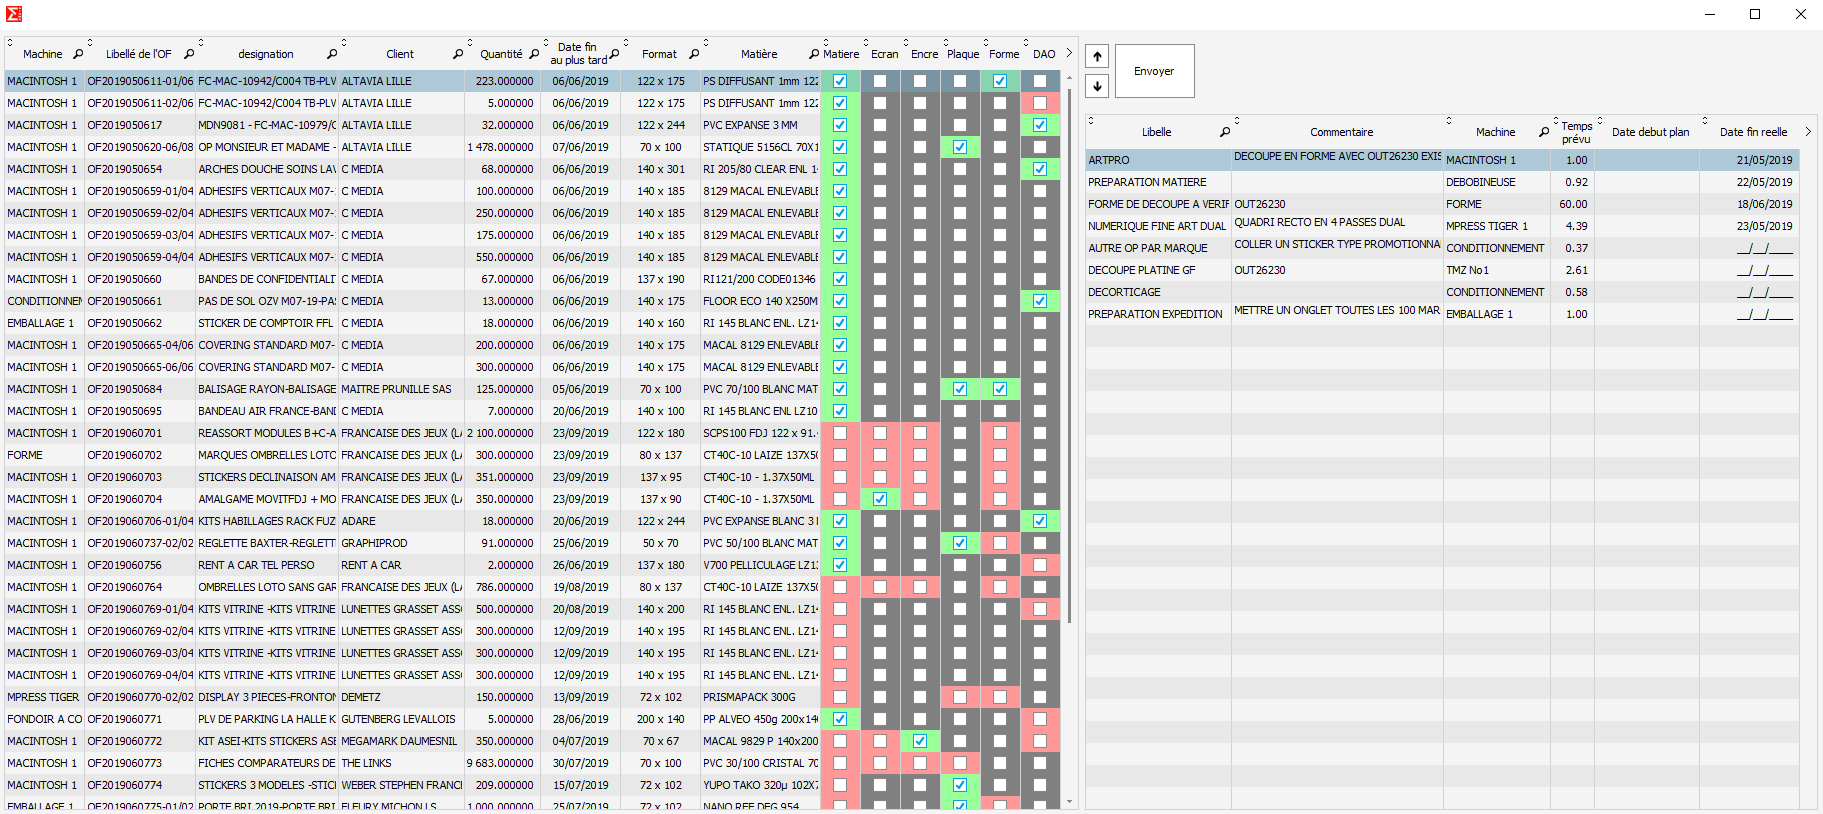
\includegraphics[width = 0.9\textwidth]{planning_2}
    \end{center}
    \caption{Aperçu de la fenêtre de tri du planning de fabrication avec l'avancement des phases de préparation}
    \label{figure:planning_2}
\end{figure}
\FloatBarrier

Le développement du planning de fabrication de \textsc{Sigma} s'est déroulé en parallèle de celui de la SFAO et il n'y a eu aucun problème majeur.

\newpage
\subsection{La SFAO de \textsc{Sigma}}

Avant le développement de \textsc{Sigma}, il existait une SFAO sur \textsc{Disanet} qui permettait de suivre le processus de fabrication de la compagnie.
Au sein de \textsc{Sigma}, nous avons décidé de développer un outil similaire, permettant de remplir le même rôle, mais en y apportant des améliorations.

\subsubsection{Le fonctionnement de l'ancienne SFAO}

Pour savoir le travail qu'ils avaient à effectuer, les ouvriers devaient se rendre au tableau de planification.
C'est ici que leur travail leur était attribué, ils devaient récupérer un dossier papier contenant l'OF, ainsi que toutes les informations nécessaires à l'impression.

Ils allaient ensuite sur un poste informatique afin d'enregistrer le début de leur phase de préparation.
Pour s'identifier, ils devaient scanner un code-barres présent sur leur badge personnel.
Ensuite, ils devaient scanner le code-barre propre à la phase de fabrication, imprimé sur le dossier papier.
Une fois la phase terminée, il fallait refaire ce même processus pour clôturer la phase.

Un système de synchronisation des données entre la SFAO et ASAP avait été mis en place, ce qui permettait de renseigner l'avancement des phases de fabrication automatiquement au sein d'ASAP.

L'objectif avec le développement de la SFAO au sein de \textsc{Sigma} était de profiter de la base de données unique pour proposer des fonctionnalités jusqu'alors impossibles et également pour diminuer la consommation de papier.

\subsubsection{Le développement de la SFAO sous \textsc{Sigma}}

J'ai effectué la quasi-totalité du développement de la SFAO.
Afin de contrôler mon travail je travaillais principalement avec M. \textsc{Mery}, responsable de la production.

La SFAO doit permettre aux ouvriers de toujours savoir le travail qu'ils ont à effectuer, en fonction de la machine sur laquelle ils travaillent.
Les ouvriers doivent pouvoir s'identifier et sélectionner leur machine facilement afin de voir les phases à faire.
La sélection de l'ouvrier et de la machine se fait simplement via une liste déroulante et les informations de phases s'affichent juste à côté de la machine sélectionnée.

Les phases s'affichent dans l'ordre de priorité défini par le planning de fabrication.
L'opérateur peut cliquer sur les phases afin d'afficher des informations complémentaires et lorsque tout est prêt il suffit de cliquer sur <<~Démarrer~>> et la phase se lance.
D'un point de vue technique lorsqu'un employé démarre une phase, un triptyque se crée en base de données, reliant la personne à la machine ainsi qu'à la phase de fabrication.
Ce triptyque permet de garder un historique complet de tout le processus de fabrication.
Il contient des informations complémentaires, telles que la date de début et de fin de la phase, les quantités préparées, des commentaires, etc.

La SFAO permet aussi de signaler les aléas, et d'en indiquer la raison.
Cela à deux intérêts, le premier est de pouvoir informer directement les responsables du souci.
Ces derniers sont informés de par l'affichage de la machine en mode erreur dans le planning et également dans le plan d'usine, un outil développé par Alexandre \textsc{Meunier} qui permet d'exploiter les données de la SFAO pour afficher un statut de toutes les machines de l'usine en direct.
Le second intérêt de signaler les aléas sur \textsc{Sigma} est l'enregistrement d'un historique en base de données.
Ce sont des données importantes qu'il faut conserver pour l'élaboration de statistiques.
Des statistiques sur les aléas des machines peuvent, par exemple, mettre en évidence une machine présentant des problèmes plus fréquemment que les autres, etc.

Enfin, un ouvrier peut suspendre une phase, pour faire une pause ou en commencer une autre pour quelque raison que ce soit.
Il peut également terminer une phase en cours et saisir les quantités préparées lors de la réalisation de celle-ci.

\FloatBarrier
\begin{figure}[h!]
    \begin{center}
        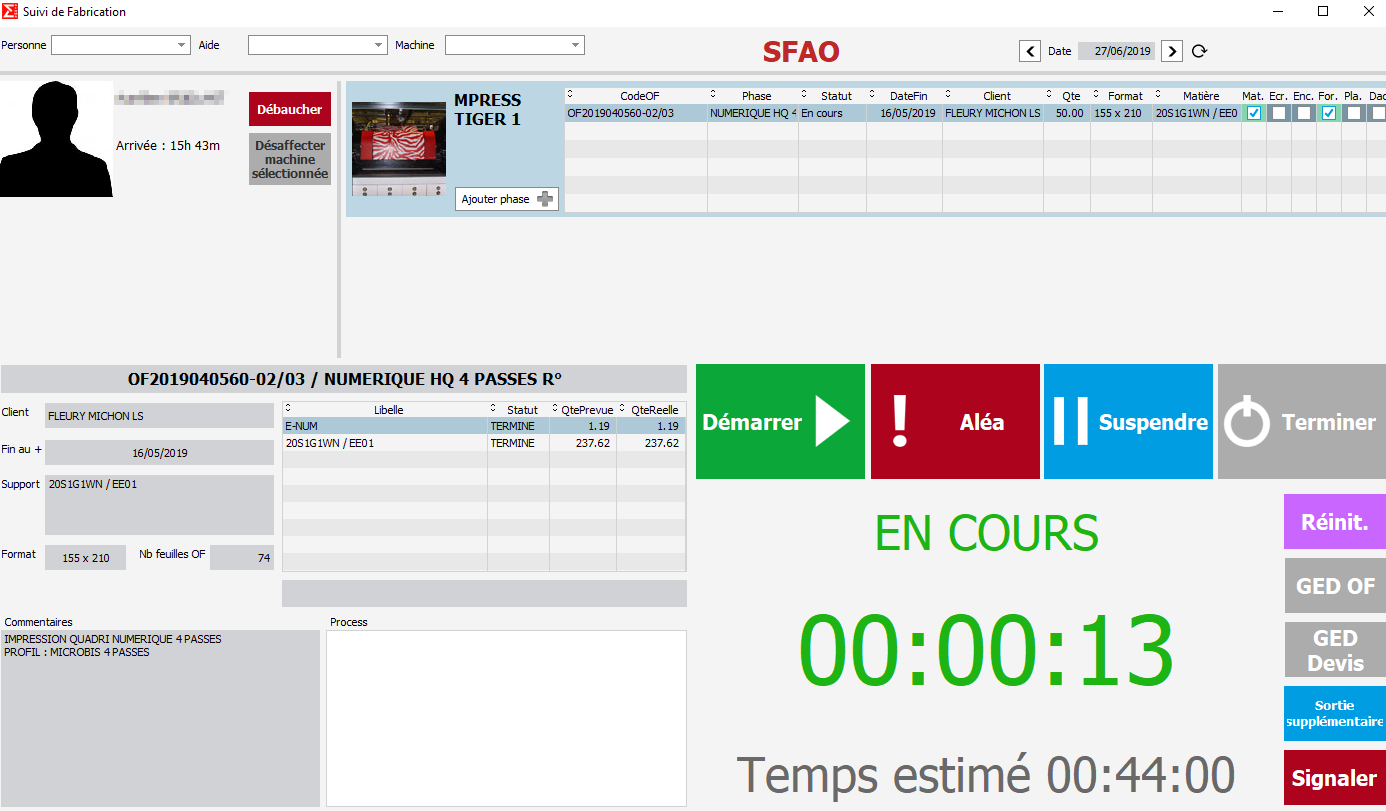
\includegraphics[width = 0.9\textwidth]{sfao}
    \end{center}
    \caption{Aperçu de la fenêtre de la SFAO, avec une phase d'impression numérique en cours}
    \label{figure:sfao}
\end{figure}
\FloatBarrier

La SFAO est un outil qui fut intéressant à développer, notamment dû au fait que nous avons réalisé son développement en parallèle avec le développement du planning de fabrication, ainsi que le plan d'usine.
Cela nous a permis à moi et Alexandre \textsc{Meunier} de développer notre capacité à travailler ensemble.

\newpage
\subsection{Module des ressources humaines}

\subsubsection{La conception du module}

Lors de ma septième mission en entreprise, il m'a été demandé de développer l'ensemble des applications permettant de gérer les absences, primes, frais professionnels, permanences, heures supplémentaires, etc.
C'est donc un module qui doit permettre des fonctionnalités variées.
Il est, dans ce cas, particulièrement important de prévoir à l'avance les différents liens entre toutes les applications, afin d'éviter des problèmes d'incohérences.

La première étape fut la préparation de la base de données.
Chaque employé possède des compteurs pour leurs congés payés de l'année en cours, ceux de l'année précédente, leurs jours d'ancienneté, etc.
Pour le développement des outils, il est nécessaire de prendre en compte la manière dont tous ces compteurs sont mis à jour.
L'ordre de développement déterminé fut tout d'abord l'outil permettant de gérer les absences, puis celui permettant de gérer les heures supplémentaires.
Une fois ces outils développés, la totalité des compteurs en base sont gérés, on peut donc développer la suite des outils sans suivre un ordre en particulier.

\FloatBarrier
\begin{figure}[h!]
    \begin{center}
        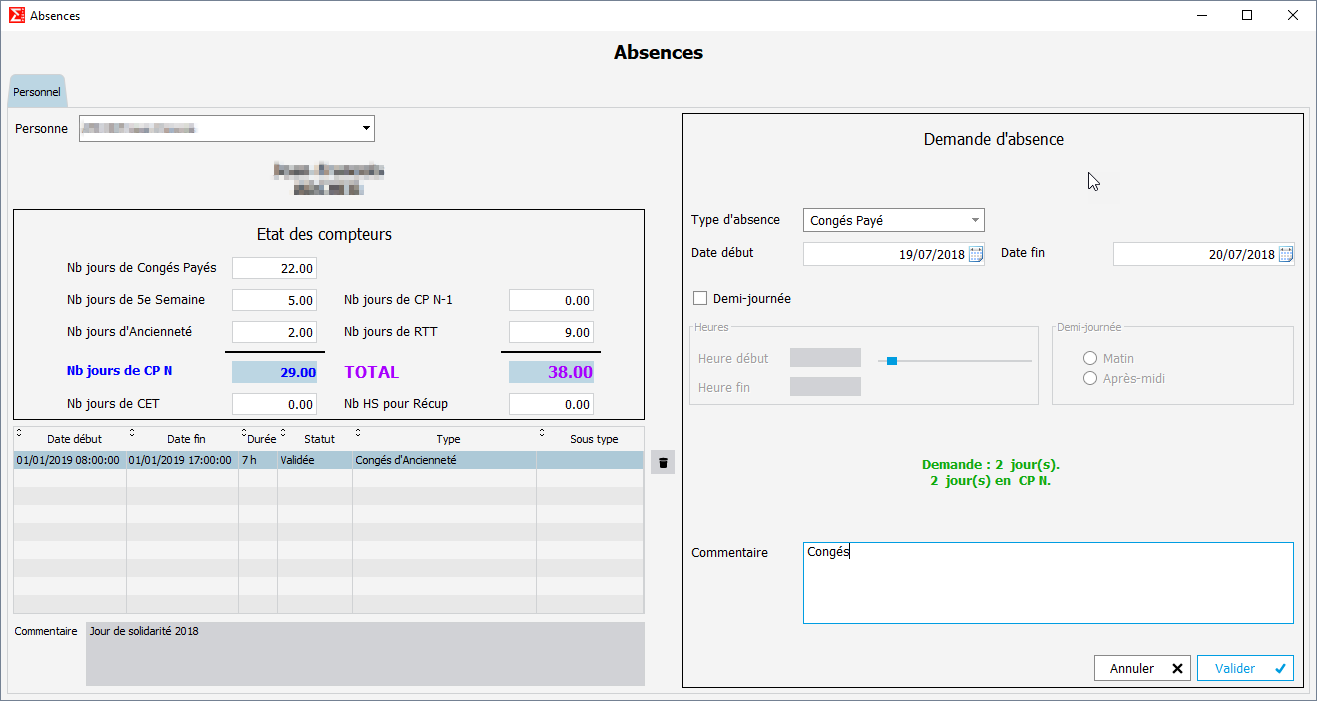
\includegraphics[width = 0.9\textwidth]{absences}
    \end{center}
    \caption{Aperçu de la fenêtre permettant de gérer ses absences}
    \label{figure:absences}
\end{figure}
\FloatBarrier

La gestion des fiches de payes est externalisée.
Chaque mois, pour tous les employés de \textsc{Disa}, un fichier \textsc{Excel} contenant toutes les informations nécessaires à la création des fiches de paie est transmis au sous-traitant.
Grâce aux nouveaux outils développés, nous avons pu automatiser la création de l'ensemble de ces fichiers en un clic.

\FloatBarrier
\begin{figure}[h!]
    \begin{center}
        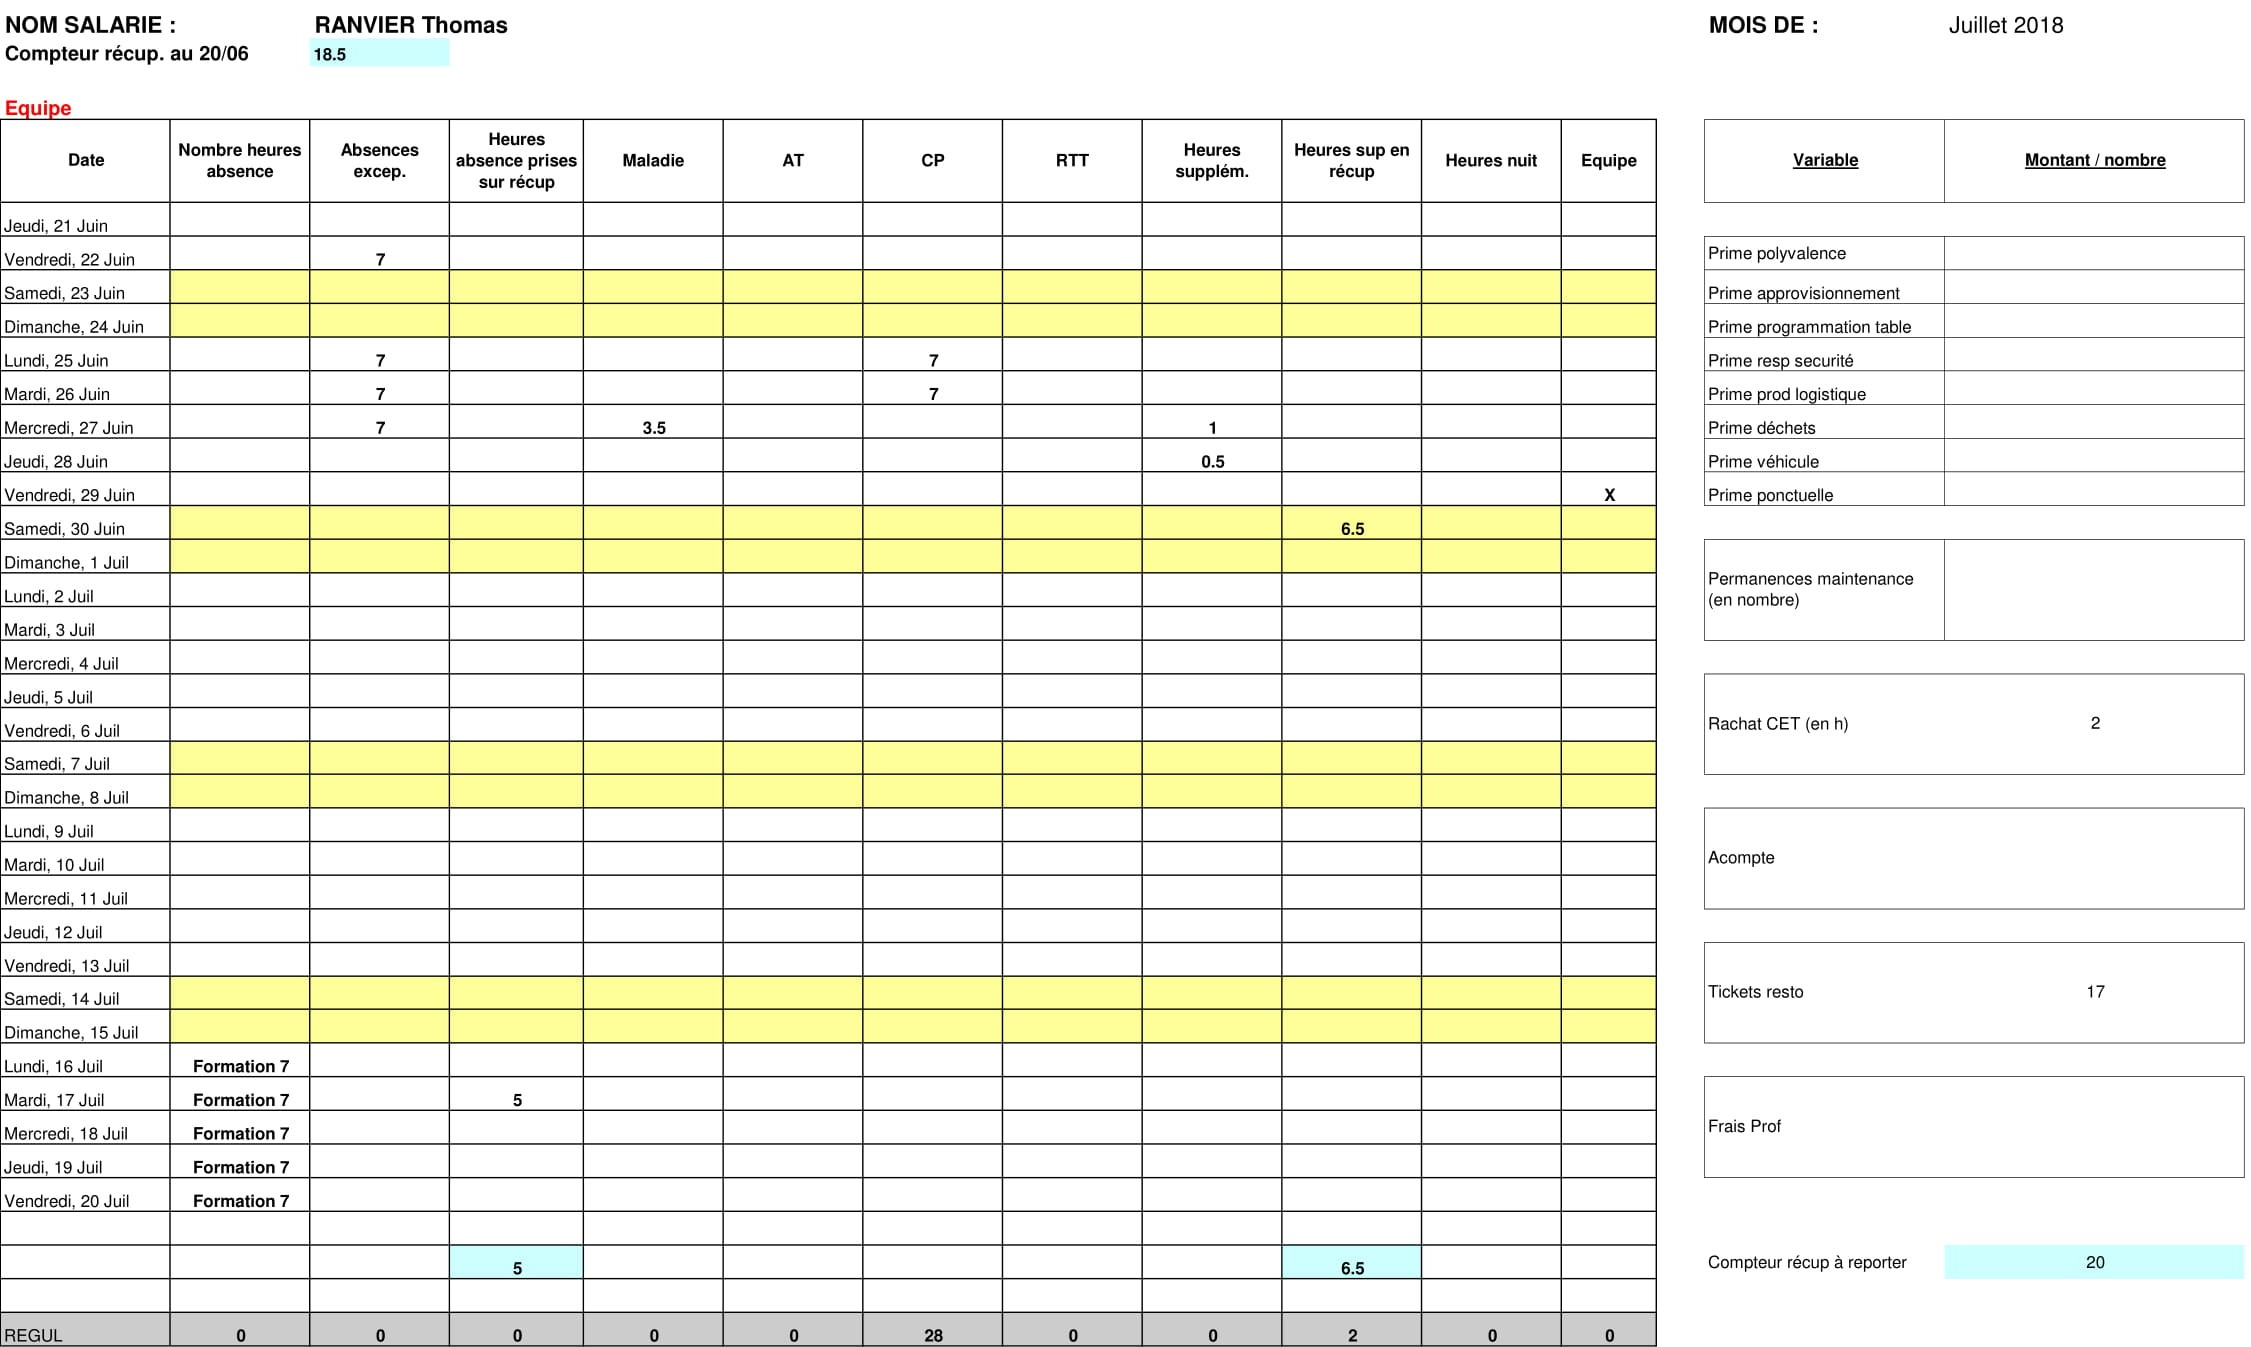
\includegraphics[width = 0.9\textwidth]{paye}
    \end{center}
    \caption{Exemple de fichier généré à partir de données fictives}
    \label{figure:paye}
\end{figure}
\FloatBarrier

\subsubsection{Les développements futurs}

Le module des ressources humaines tel qu'il est développé actuellement ne permet pas de gérer les congés dans le respect complet des lois.
Le principal problème est que les droits à des jours de congés ne sont actualisés qu'une fois par an alors que les congés acquis chaque mois devraient être automatiquement ajoutés aux compteurs des employés.
Cela a pour effet d'obliger les employés à poser des congés par anticipation au sein de \textsc{Sigma} alors que ce sont en fait des congés qu'ils ont acquis au cours de l'année.

La correction de ce souci peut sembler plutôt simple d'un œil extérieur, mais en fait l'adaptation du module des ressources humaines à ce fonctionnement entraînerait beaucoup de modifications nécessaires pour retrouver un fonctionnement stable.
Nous sommes donc actuellement en réflexion avec M. \textsc{Stecleboute}, le nouveau responsable informatique, pour trouver la meilleure manière de s'y prendre pour mettre à jour ce système.

\newpage
\subsection{Mon travail lors de cette dernière mission}

La fin de la mise en production de \textsc{Sigma} s'est effectuée en grande partie lors de mon séjour à l'étranger, je n'étais donc pas présent.
Beaucoup d'employés utilisaient déjà \textsc{Sigma} au quotidien avant cette fin de mise en production, puisque celle-ci s'est effectuée graduellement dans le temps.
Durant la période de fin d'année 2018, M. \textsc{Palier} et M. \textsc{Stecleboute} ont formés les employés qui n'utilisaient pas encore \textsc{Sigma}.

Lors de cette dernière mission, le travail que j'ai eu à réaliser était donc principalement de la correction de bug, la modification et l'amélioration de certaines fonctionnalités afin de mieux les adapter aux besoins des utilisateurs et aussi le développement de quelques nouvelles fonctionnalités.

\subsubsection{Amélioration de la gestion du travail au sein du service informatique}

Afin de gérer les corrections de bugs nous avons mis en place une adresse mail sur laquelle les utilisateurs peuvent nous faire parvenir tous les soucis qu'ils rencontrent.
Afin de simplifier la gestion de ces corrections en tant qu'équipe, j'ai proposé d'utiliser l'outil de gestion de projet \textsc{Trello}.
Nous avons synchronisé la boîte mail des bugs avec cet outil, ainsi dès qu'un mail est reçu, une tâche est créée au sein de \textsc{Trello}.
Les tâches créées au sein de \textsc{Trello} peuvent être attribuées à une personne, il est possible de les commenter, les déplacer dans différentes catégories, etc.
L'utilisation de cet outil a permis de simplifier notre gestion du travail au sein du service informatique.
Désormais lorsque nous voulons développer une nouvelle fonctionnalité ou en améliorer une ancienne, on y crée une tâche qui permet de suivre l'avancement du travail.
\textsc{Trello} nous permet aussi de garder un historique simple à parcourir dans lequel on peut retrouver des informations concernant différentes tâches réalisées plus tôt.

\FloatBarrier
\begin{figure}[h!]
    \begin{center}
        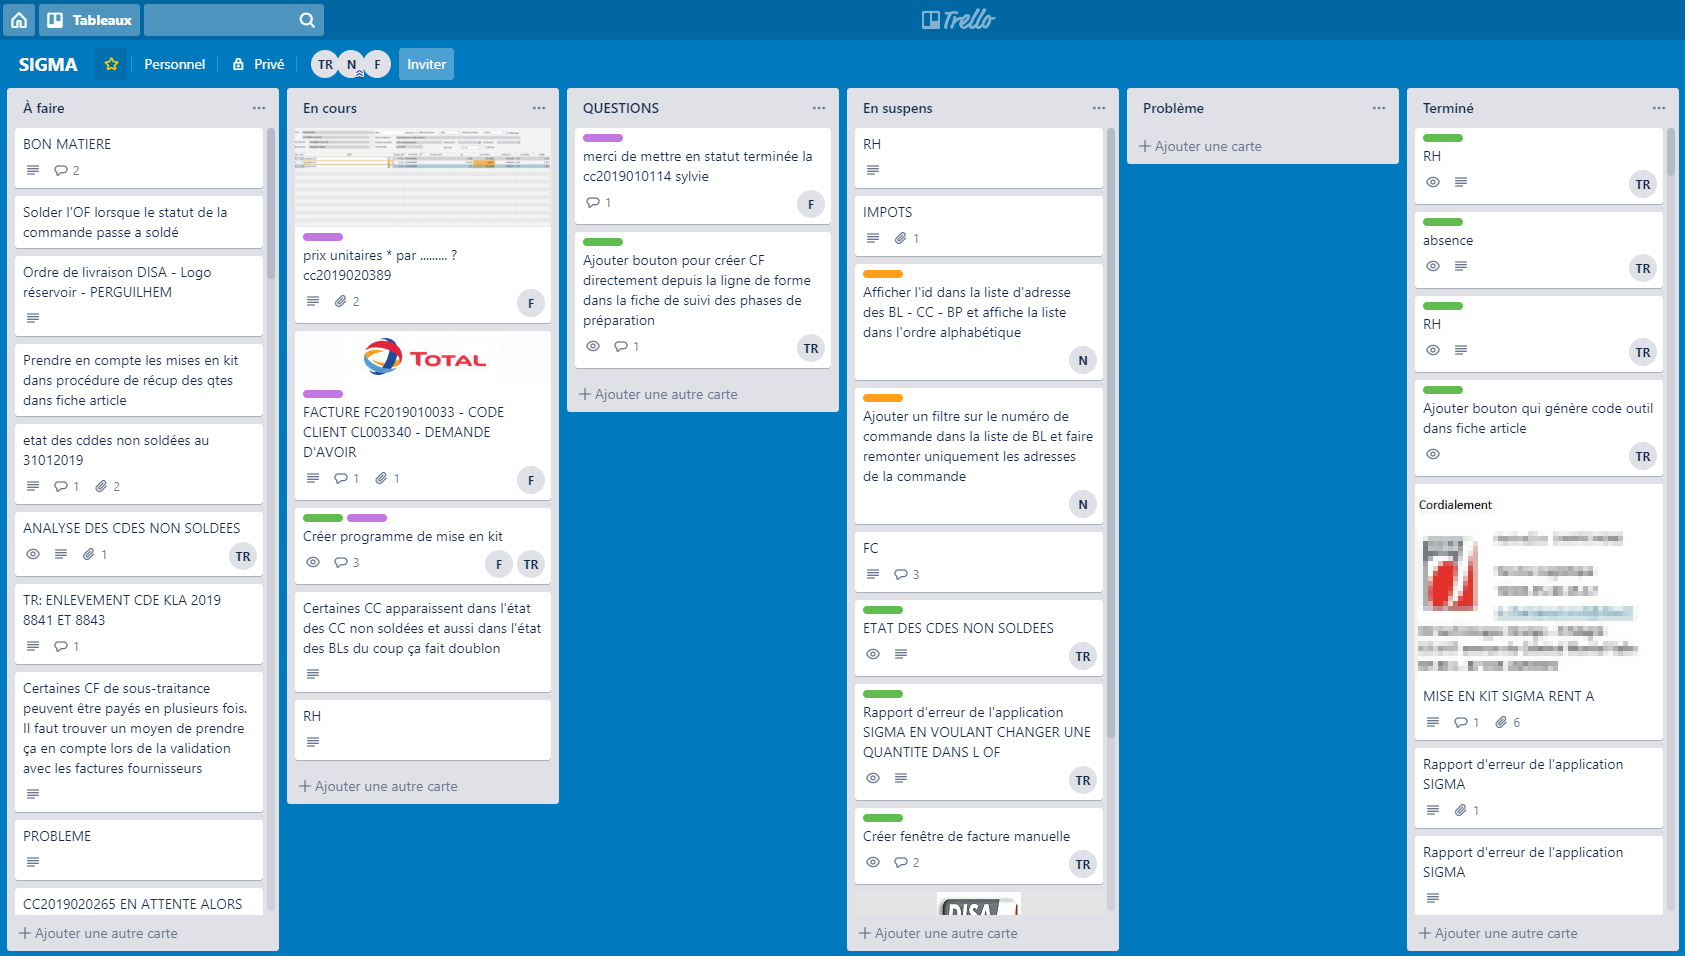
\includegraphics[width = 0.9\textwidth]{trello}
    \end{center}
    \caption{Aperçu du tableau du projet \textsc{Sigma} sous \textsc{Trello}}
    \label{figure:trello}
\end{figure}
\FloatBarrier

\subsubsection{Amélioration des performances des requêtes}

Lors du développement de certaines fenêtres permettant l'affichage de données pour des statistiques nous nous sommes aperçus que certaines requêtes en base de données étaient particulièrement longues à exécuter.
Après quelques recherches, nous avons découvert avec M. \textsc{Stecleboute} que les requêtes utilisant le Wlangage étaient plus longues à exécuter que les requêtes SQL.
En remplaçant certaines de ces anciennes requêtes par des requêtes SQL nous avons noté une amélioration de performances par un facteur de 2, voire 3.

Il s'avère que nous n'avions jamais remarqué cette différence notable de performance plus tôt puisque les requêtes habituelles étaient bien moins conséquentes et avaient donc un temps d'exécution négligeable par rapport aux requêtes nécessaires pour l'affichage de ces statistiques.
Nous avons donc remplacé beaucoup de requêtes écrites avec le Wlangage par leur équivalent en SQL afin d'améliorer les performances de celles-ci.
Désormais lorsque nous faisons des requêtes en base de données nous nous efforçons de toujours les écrire en SQL.

\subsubsection{Nouvelles fonctionnalités}

Au cours de cette dernière mission, la très grande majorité de mon travail était concentrée sur la résolution de bugs rencontrés par les employés et l'amélioration de fonctionnalités permettant de faciliter leur travail quotidien.

Une autre partie de mon travail fut aussi de développer des fonctionnalités jusqu'alors inexistantes.
J'ai notamment développé une application permettant de gérer les mises en kits\footnote{Les mises en kits consistent en le conditionnement et l'expédition de produits déjà fabriqués.}.
Il fallait donc développer une application permettant de facilement connaître l'état des stocks de tous les composants du kit à envoyer.

J'ai aussi développé, avec M. \textsc{Stecleboute}, des fonctionnalités permettant la gestion des formes de découpes.
Jusqu'à présent, la gestion des formes de découpes se faisait encore à l'aide de \textsc{Disanet}.
Les formes de découpes possèdent un statut qui leur est propre, il est aussi important de sauvegarder le devis de fabrication de chaque forme, etc.
Les formes de découpes sont un type particulier d'article, or tous les types d'articles sont gérés au sein de \textsc{Sigma}.
Nous avons donc adapté le module de gestion des articles afin de prendre en compte les particularités des formes de découpes.
Désormais, elles peuvent être entièrement gérées avec \textsc{Sigma}.

\newpage
\section{Retour d'expérience sur mon apprentissage}

Mon apprentissage au sein de la compagnie \textsc{Disa} fut enrichissant de par la diversité des tâches que j'ai eu à effectuer.

J'ai principalement travaillé sur le projet \textsc{Sigma}, qui est un projet de grande ampleur qui s'est déroulé sur la totalité de mon apprentissage.
J'ai effectué des tâches de récolte du besoin, analyse du besoin, conception, développement, puis déploiement de l'ERP.
C'est donc un travail très diversifié, demandant de la réflexion et qui m'a permis d'acquérir des connaissances et une expérience qui me sera précieuse.

Le projet \textsc{Sigma} peut être considéré comme un succès.
La totalité des employés de la compagnie l'utilisent au quotidien et il leur permet d'effectuer leur travail plus facilement et dans de meilleures conditions qu'auparavant.
Le travail de correction des bugs a permis de se débarrasser de tous les problèmes empêchant les employés de travailler correctement, cependant, il reste de nombreux points à améliorer.
Ce travail devra donc se poursuivre jusqu'à l'obtention d'un ERP stable ne nécessitant que des modifications exceptionnelles.

Bien sûr, il y aura toujours de nouvelles applications à développer ou à modifier sur \textsc{Sigma} afin de l'adapter aux besoins changeants des employés.

Je suis, dans l'ensemble, satisfait par mon travail sur ce projet.